\begin{figure}[t]
  \centering
  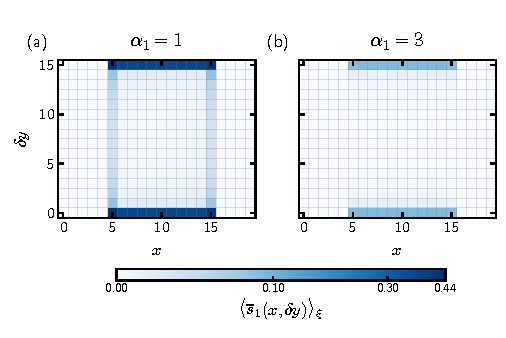
\includegraphics[width=\columnwidth]{entropy_contours_hard_n20x32_alpha1_1_3_y0avg.pdf}
  \caption{\textbf{Origin-averaged entanglement contours.}
  Von Neumann entanglement contours for (a) $\alpha_1=1$ and
  (b) $\alpha_1=3$, at $N_x=20$, $N_y=32$, $\alpha_2=30$, and
  cycle $64=2N_y$. The hard-wall circuit uses $n_{\mathrm{shell}}=1$,
  raster-$y$ ordering, and perfect correction, starting from random
  half-filled pure states with Born-conditioned exterior preparation.
  For each of $100$ independent trajectories per panel, the contour is
  computed on $[0,20)\times[y_0,y_0+16)$ for every periodic origin
  $y_0=0,\ldots,31$. Cuts are aligned by $\delta y=(y-y_0)\bmod N_y$
  and averaged within each trajectory before averaging trajectories.
  Each pixel sums both orbitals. Both panels share the same square-root
  Blues normalization; gray lines mark unit cells.}
  \label{fig:entropy-contour-alpha-comparison-y0avg}
\end{figure}
